\chapter{Neutron Partonic Structure}
\label{chap:physics}

\section{Physics motivations: Neutron GPDs}

A wealth of information on the structure of hadrons lies in the correlations 
between the momentum and spatial degrees of freedom of the partons. These 
correlations can be revealed through deeply virtual Compton scattering (DVCS), 
i.e., the hard exclusive lepto-production of a real photon, which provides 
access to a three-dimensional (3-D) imaging of partons within the generalized 
parton distributions (GPDs) framework 
\cite{Mueller:1998fv,PhysRevLett.78.610,PhysRevD.55.7114,Radyushkin:1996nd,PhysRevD.56.5524}.   
The measurement of free proton DVCS has been the focus of a worldwide effort 
\cite{PhysRevLett.87.182002,
   PhysRevLett.87.182001,
   PhysRevD.75.011103,
   Girod:2007aa,
   PhysRevC.92.055202,
   PhysRevLett.99.242501,
   PhysRevC.80.035206,
   PhysRevLett.114.032001,
   Jo:2015ema}
involving several accelerator facilities such as Jefferson Lab, DESY and  
CERN. These measurements now enable the extractions of GPDs and a 3-D 
tomography of the free proton \cite{Guidal:2013rya, PhysRevD.95.011501}. The 
aim of this proposal is enhance the neutron GPD measurements along the approved 
CLAS12 experiment E12-11-003, which will also measure the quasi-free neutron 
DVCS by detecting the scattered neutron in deuterium.  

In the fits of PDFs, \cite{Ball:2014uwa} for example, neutrino and deuterium data allow to make
a flavor dependent extraction, this option is not available for GPDs yet due to 
the lack of reliable data. Indeed, the observables of DVCS, such as cross sections
and beam-spin asymmetries are much smaller on neutron targets, while the nuclear
effects in deuterium increase uncertainties. These issues have lead to results
\cite{Mazouz:2007aa} which are not precise enough to help in a flavor dependent GPD extraction.
To achieve this performance, one will need a large quantity of high precision data
a goal set by the E-12-11-003. However, the impact of the uncertain initial state and the
final state interactions on the integration of these data in global fits remain 
unclear. With this proposal, we propose to both provide more data on the neutron,
which is always important, but most importantly these data will have completely 
independent systematic errors from the E-12-11-003 data. That will make them complementary
and indicate in what ways these methods are equivalent or potentially need {\it ad hoc}
corrections.

Neutron DVCS is also hoped to provide an important contribution to the 
extraction of the GPD $E$~\cite{dHose:2016mda}. The reasoning behind this expectation is as 
follows, the GPD $E$ never appears to be dominant in usually measured DVCS 
observables, as a sub-leading contribution it is always plagued with large 
error bars. Actually, recent extractions \cite{Dupre:2017hfs,Moutarde:2018kwr} show 
that we still barely have any constraint on $E$ using all the world proton 
data.  However, as form factors often appear in the expressions of
DVCS observables because of the Bethe Heitler process (see below) the situation 
is very different for protons and neutrons. Indeed, the $F_1$ form factor of the 
neutron is very small, making the $E$ GPD more prominent in some of the neutron DVCS 
observables. Most notably the $\sin$ component of the beam spin asymmetry 
(see Eq. \ref{eq:sin} below for details) is given 
by~\cite{dHose:2016mda}:
\begin{equation}
s^\textrm{I}_{1,\textrm{unp}} \propto \Im m \left [ 
F_1 \mathcal{H} + \xi(F_1 + F_2) \mathcal{\tilde H} - \frac{t}{4M^2} F_2  \mathcal{E} \right ],
\end{equation}
highlighting the effect of a suppressed $F_1$ on the main term.
This lead to the idea that neutron DVCS will also help significantly to constrain the 
GPD $E$. This goal is of course driven by the long standing objective of GPD physics to
measure the Ji sum rule in the nucleon:

\begin{equation}
J_q \,=\, {1 \over 2} \, \int_{-1}^{+1} d x \, x \, 
\left[ H^{q}(x,\xi,t = 0) + E^{q}(x,\xi,t = 0) \right],
\label{eq:dvcs_spin}
\end{equation}
which links the total angular momentum ($J_q$) carried by each quark $q$ to the 
sum of the second moments over $x$ of the GPDs $H$ and $E$, that will complete 
the decomposition of the nucleon spin in its various components 
\cite{PhysRevLett.78.610}. 

\section{DVCS Formalism and Observables}

The cross section for DVCS on a spin-1/2 target can be parameterized in terms 
of four helicity conserving GPDs: $H^q$, $E^q$, $\tilde{H}^q$, and 
$\tilde{E}^q$. The GPDs $H$, $E$, $\widetilde{H}$ and $\widetilde{E}$ are 
defined for each quark flavor (q = u, d, s, ... ). Analogous GPDs exist for the 
gluons, see references \cite{Ji:1996ek,PhysRevD.56.5524,Goeke:2001tz} for details.  In 
this work, we are mostly concerned by the valence quark region, in which the 
sea quarks and the gluons contributions do not dominate the DVCS scattering 
amplitude. The GPDs $H$ and $\widetilde{H}$ conserve the spin of the nucleon, 
while $E$ and $\widetilde{E}$ flip it. The $H$ and $E$ GPDs are called the 
unpolarized GPDs as they represent the sum over the different configurations of 
the quarks' helicities, whereas $\widetilde{H}$ and $\widetilde{E}$ are called 
the polarized GPDs because they are made up of the difference between the 
orientations of the quarks' helicities.

\begin{figure}
   \centering
   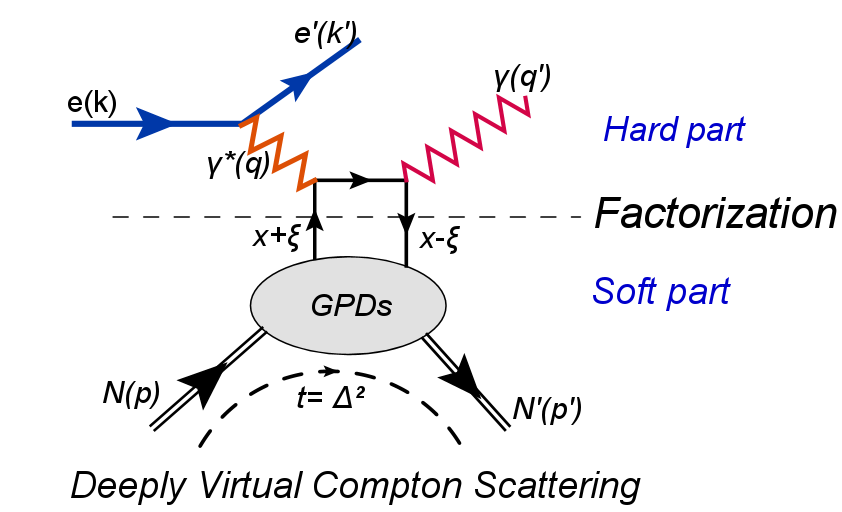
\includegraphics[width=0.60\textwidth,,clip,trim=0mm 20mm 0mm 0mm 
   ]{figures/DVCS2.png}
   \caption{\label{fig:dvcshandbag} Leading-twist DVCS handbag diagram with the 
   momentum definitions labeled.}
\end{figure}

The differential cross section of leptoproduction of photons for a 
longitudinally-polarized electron beam and an unpolarized nucleon target can 
be written as:
\begin{equation}
\frac{d\sigma}{dx_B\,dy\,dt\,d\phi\,d\varphi} = \frac{\alpha^3 x_B y}{16 \pi^2 
   Q^2 \sqrt{1+\epsilon^2}} \left| \frac{\mathcal{T}}{e^3} \right|^2
\end{equation}
where $\epsilon \equiv 2x_B \frac{M_n}{Q}$, $x_B=Q^2/(2p_1\cdot q_1$) is the 
Bjorken variable, $y= (p_1\cdot q_1)/(p_1\cdot k_1)$ is the photon energy 
fraction, $\phi$ is the angle between the leptonic and hadronic planes, 
$\varphi$ is the scattered electron's azimuthal angle, $Q^2= -q_1^2$, and 
$q_1=k_1-k_2$. The particle momentum definitions are shown in 
Figure~\ref{fig:dvcshandbag}. The momentum transfer where the nucleon is 
initially at rest, $\Delta = p_1-p_2$ and $t=\Delta^2$. The Bjorken variable  
is related to another scaling variable called skewedness:
\begin{equation}
\xi = \frac{x_B}{2 - x_B} + \mathcal{O}(1/Q^2).
\end{equation}

The amplitude is the sum of the DVCS, the Bethe-Heitler (BH), and the 
interference amplitudes, and when squared has terms
\begin{equation}
   \mathcal{T}^2 = \left|\mathcal{T}_{\text{BH}}\right|^2 + 
   \left|\mathcal{T}_{\text{DVCS}}\right|^2 + \mathcal{I}
\end{equation}
where the first is the BH contribution, the second is the DVCS part, and the last 
term is the interference part,
\begin{equation}
   \mathcal{I} = \mathcal{T}_{\text{DVCS}}\mathcal{T}_{\text{BH}}^{*} + 
   \mathcal{T}_{\text{DVCS}}^{*}\mathcal{T}_{\text{BH}}.
\end{equation}
The corresponding amplitudes are calculated with the diagrams shown in Figures 
\ref{fig:dvcshandbag} and \ref{fig:BHhandbag}. The details of contracting the 
DVCS tensor with various currents and tensors can be found 
in~\cite{Kirchner:2003wt}.
\begin{figure}[!hbt]
   \centering
   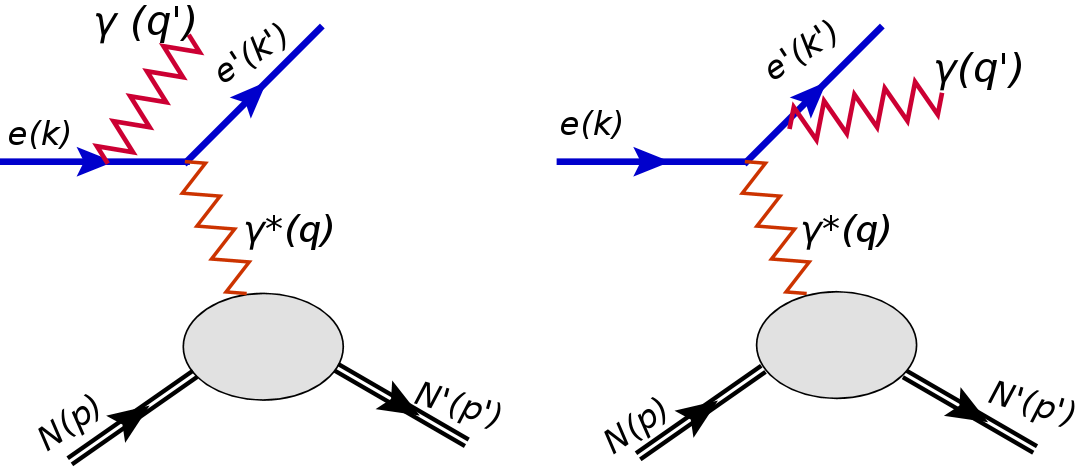
\includegraphics[width=0.65\textwidth]{figures/BH.png}
   \caption{\label{fig:BHhandbag} BH handbag diagrams.}
\end{figure}
%
The resulting expressions for the amplitudes are
\begin{align}
   \left|\mathcal{T}_{\text{BH}}\right|^2 &= 
   \frac{e^6(1+\epsilon^2)^{-2}}{x_B^2\,y^2\,t\,
   \mathcal{P}_1(\phi)\mathcal{P}_2(\phi)} \left\{ c_0^{\text{BH}} + 
   \sum_{n=1}^{2}\left[ c_n^{\text{BH}}\cos(n\phi) +s_n^{\text{BH}}\cos(n\phi) 
\right] \right\} \\
\left|\mathcal{T}_{\text{DVCS}}\right|^2 &= \frac{e^6}{y^2\,Q^2}\left\{ 
c_0^{\text{DVCS}} + \sum_{n=1}^{2}\left[ c_n^{\text{DVCS}}\cos(n\phi) 
+s_n^{\text{DVCS}}\cos(n\phi) \right] \right\}\\
   \mathcal{I} &= \frac{e^6(1+\epsilon^2)^{-2}}{x_B\,y^3\,t\,
   \mathcal{P}_1(\phi)\mathcal{P}_2(\phi)}\left\{ c_0^{\mathcal{I}} + 
   \sum_{n=1}^{3}\left[ c_n^{\mathcal{I}}\cos(n\phi) 
+s_n^{\mathcal{I}}\cos(n\phi) \right] \right\}
	\label{eq:sin}
\end{align}
%
The functions $c_0$, $c_n$, and $s_n$ are called \emph{Fourier coefficients} 
and they depend on the kinematic variables and the operator decomposition of 
the DVCS tensor for a target with a given spin. At leading twist there is a 
straightforward form factor decomposition which relates the vector and 
axial-vector operators with the so-called Compton form factors 
(CFFs)~\cite{Belitsky:2000gz}. The Compton form factors appearing in the DVCS 
amplitudes are integrals of the type
%
%
\begin{equation}
   \mathcal{F} = \int_{-1}^{1} dx F(\mp x,\xi,t) C^{\pm}(x,\xi)
\end{equation}
where the coefficient functions at leading order take the form
\begin{equation}
   C^{\pm}(x,\xi) = \frac{1}{x-\xi + i\epsilon} \pm \frac{1}{x+\xi - 
   i\epsilon}.
\end{equation}
%
We plan on measuring the beam spin asymmetry as a function of $\phi$
\begin{equation}
   A_{LU}(\phi) = \frac{d\sigma^{\uparrow}(\phi) - 
   d\sigma^{\downarrow}(\phi)}{d\sigma^{\uparrow}(\phi) + 
   d\sigma^{\downarrow}(\phi)}
\end{equation}
%
where the arrows indicate the electron beam helicity. 

\section{Measuring the neutron DVCS}

\subsection{Two new methods for two objectives}

As shown in Fig.~\ref{fig:ndvcsexclusive}, one can measure all the components of 
the DVCS reaction on deuterium using CLAS and Bonus12. This method, while perfect 
on the paper, leads to an efficiency problem
as both the measurement of the spectator proton and of the neutrons are challenging
and low efficiency (intrinsically for the neutron and by the limitation of phase 
space available for the proton). However, it is possible to ensure the exclusivity
of a process when missing one of the final state particles by applying cuts on
missing mass, momentum and energy. This strategy can be used, either to leave the
spectator proton or the neutron undetected. The former, being used in the ongoing
E-12-11-003. We propose here to perform the other option, detecting the spectator proton
but not the neutron, in order to increase the amount of available data, but most 
importantly, to confirm the equivalency of both methods. Moreover, we will be able to
perform the fully exclusive measurement, but with rather limited statistics. We
intend to use this over-constrained last measurement to study the systematic effects 
linked to the nuclear target and the uncertainties in detection.

\begin{figure}
   \centering
   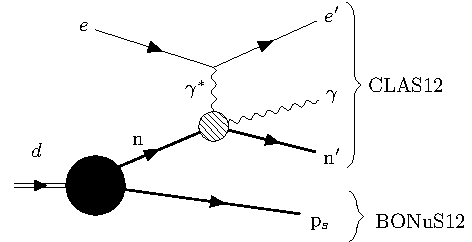
\includegraphics[width=0.60\textwidth,,clip,trim=0mm 0mm 0mm 0mm 
   ]{figures/dvcs_feynman-figure1.pdf}
   \caption{\label{fig:ndvcsexclusive} Fully exclusive neutron DVCS diagram in 
   deuterium. }
\end{figure}

\subsection{Tagged neutron DVCS with BONuS12}

The tagged neutron detection scheme is described in Fig.~\ref{fig:ndvcstagged}, where we see
that a detector for low energy proton spectators is necessary. Here, we propose to use the 
Bonus radial TPC, which is designed to make a similar type of measurement for inclusive 
deeply inelastic scattering. The first goal of the present proposed experiment is simply
to provide more data in the field of neutron GPD. Indeed, the measurement of neutron
DVCS is very challenging and very little published data is available at this point. 

\begin{figure}
   \centering
   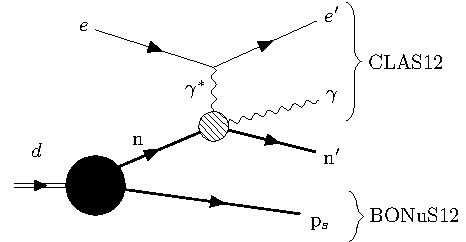
\includegraphics[width=0.60\textwidth,,clip,trim=0mm 0mm 0mm 0mm 
   ]{figures/dvcs_feynman-figure0.pdf}
   \caption{\label{fig:ndvcstagged} Neutron Tagged-DVCS diagram in deuterium.  
   }
\end{figure}

Second, we observe that the systematics from this measurement are going to be mostly 
independent of the ones from E-12-11-003. Indeed, while this measurement will be missing one 
of the high energy product of the reaction leading to more uncertainty in exclusivity cuts,
it will detect the spectator proton, significantly help with nuclear effects. This has interestingly
an impact on both initial state and final state effects. In the initial state, the neutron is
in fact not at rest and carries some Fermi momentum, which can be directly inferred from the
kinematic of the spectator proton, thanks to the simple two body deuterium. On the final state side,
detecting the spectator proton in a certain range of momentum and angle allows to significantly 
reduce the probability of final state interactions to have occurred.

In order to resolve the initial state issue, we evaluate the standard Lorentz invariant 
$x$ in terms of the spectator kinematics. $x$ acquires a star to indicate  true 
invariants rather than the values calculated assuming a stationary, on-shell 
target:
\begin{equation}
   x^* = \frac{Q^2}{2M_{N}Ey (2-\alpha_s} = \frac{x_B}{2-\alpha_s},
\end{equation} 
where $\alpha_s = \frac{E_s - p^{z}_{s}}{M_N}$, with $M_N$, $E_s$, and 
$p^{z}_{s}$ are the on-shell mass, energy, and z-momentum component of the 
spectator proton. 

To understand the regions where final state interactions are expected to be significant, we
look at the spectator momentum 
and angle relative to the momentum transfer, $\theta_s$. In 
Fig.~\ref{fig:deuteronFSI}~\cite{CiofidegliAtti:2003pb,CiofidegliAtti:2002as}, we
see calculations for the inclusive case.  
At low recoil momentum and backwards spectator angle, the FSIs are negligible, 
where at high momenta perpendicular to the momentum transfer, the FSIs are 
maximized.

\begin{figure}
   \centering
   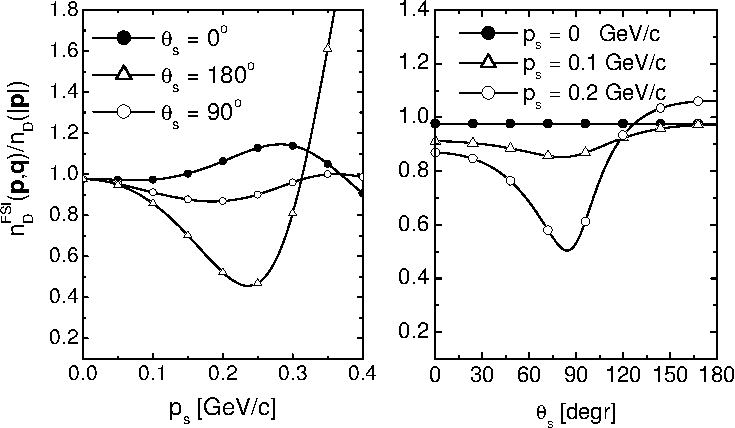
\includegraphics{figures/FSI_quasielastic_Atti_2003.pdf}
   \caption{\label{fig:deuteronFSI} Ratio of cross sections for the FSI model 
   from~\cite{CiofidegliAtti:2003pb} to PWIA calculation as a function of
   the spectator momentum (left) and spectator angle (right).}
\end{figure}

It is important to note that the detection of the neutron or the spectator proton are not equivalent.
While it could appear to be so after applying the exclusivity cut, it is not the case because of the 
large uncertainty (a percent or more) in the energy measurement of photons. This uncertainty is larger
than the momentum of the spectator proton and therefore completely hinders our capability to reconstruct
it, if it is not directly measured.
In conclusion, the measurement of this channel will offer a similar amount of data as other 
CLAS12 measurements but with different systematic effects. In particular, reducing the impact
of the least known nuclear effects.

\subsection{Fully exclusive neutron DVCS with BONuS12}

As highlighted above, the fully exclusive measurement of neutron DVCS is plagued by
two difficult particles to measure, a slow proton and a fast neutron. However, it can 
still provide relevant information in a limited kinematic space. As this measurement is
fully exclusive, it provides over-constraints by using missing mass, momentum and energy 
cuts. This will give us a particularly clean sample of data with a minimal amount of 
corrections to be applied and the bast control over systematic errors. We propose to use 
this sample, that can only be obtained using a recoil detector, to study the effects 
described above of Fermi motion, final state interactions and incomplete detection of the
final state. This will confirm assumptions made in other neutron DVCS measurements and
help understand better their systematic errors.



